%\documentclass[notes]{beamer}       % print frame + notes
%\documentclass[notes=only]{beamer}   % only notes
\documentclass{beamer}              % only frames
%
% Choose how your presentation looks.
%
% For more themes, color themes and font themes, see:
% http://deic.uab.es/~iblanes/beamer_gallery/index_by_theme.html
%
\mode<presentation>
{
  \usetheme{Madrid}      % or try Darmstadt, Madrid, Warsaw, ... default
  \usecolortheme{beaver} % or try albatross, beaver, crane, ... default
  \usefonttheme{default}  % or try serif, structurebold, ...
  \setbeamertemplate{navigation symbols}{}
  \setbeamertemplate{caption}[numbered]
} 

\usepackage[english]{babel}
\usepackage[utf8x]{inputenc}
\usepackage{caption}
\usepackage{booktabs}  % to make professional tables


\title[sip]{Group project}
%\subtitle{bla}
\author{Sandro Boccuzzo, No\" elle Schenk}
%\date{bla}


\begin{document}

{\usebackgroundtemplate{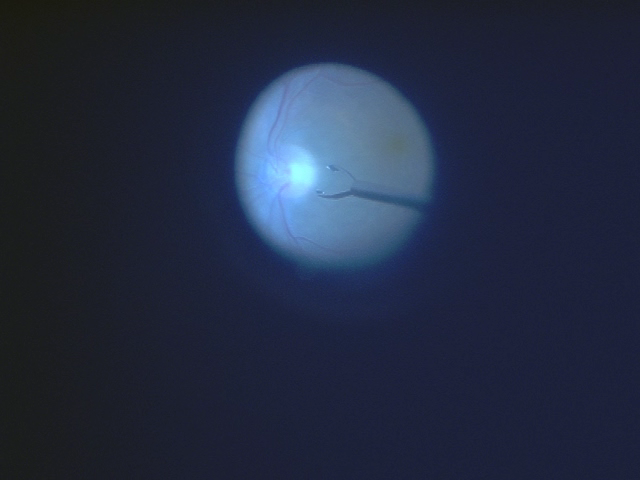
\includegraphics[width=1.0\paperwidth]{figs/title.png}}
  \begin{frame}
  \titlepage
  \end{frame} }



% ---------------------------------------------------------------------------------
\begin{frame}{simplest approach}
Filter with template cut around previous location. Problem around picture a267:
\begin{figure}
    \centering
    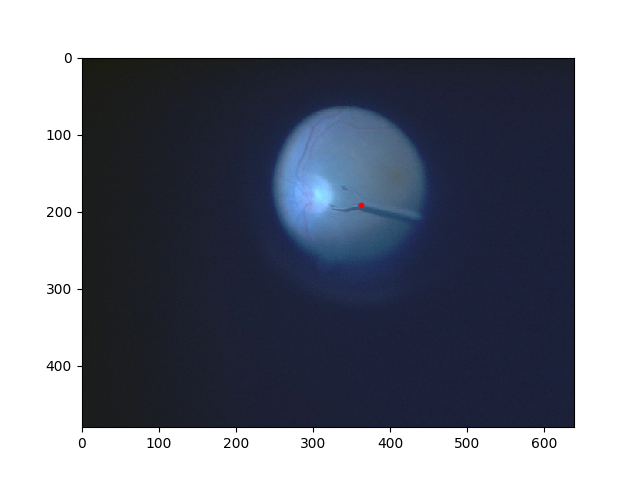
\includegraphics[width=0.25\textwidth]{figs/simplest/000267.png}
    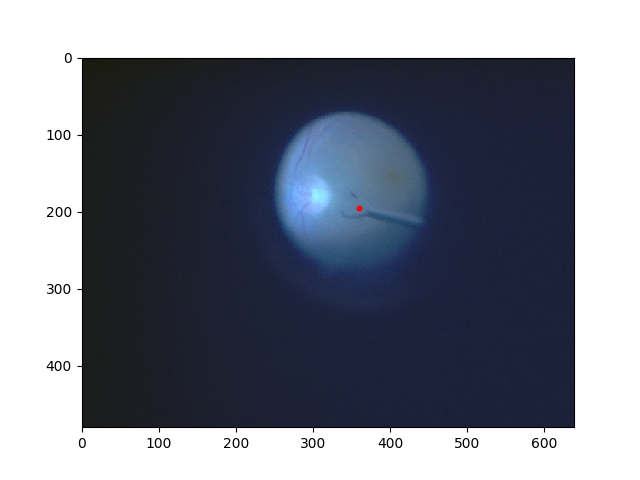
\includegraphics[width=0.25\textwidth]{figs/simplest/000268.png}
    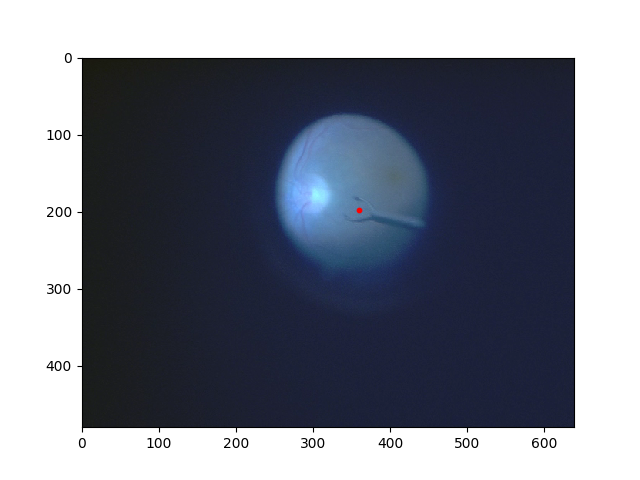
\includegraphics[width=0.25\textwidth]{figs/simplest/000269.png}
    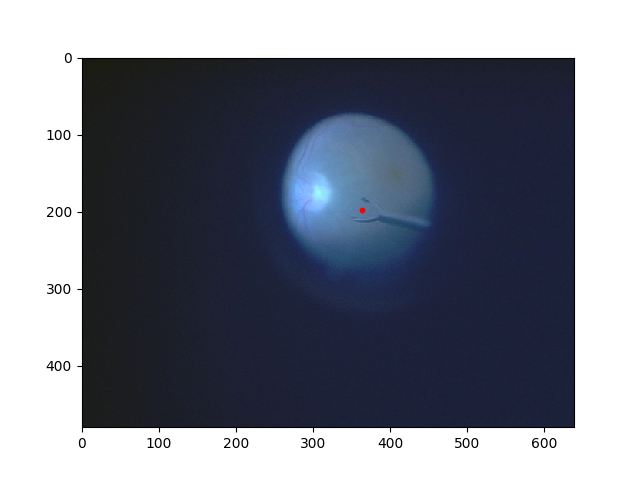
\includegraphics[width=0.25\textwidth]{figs/simplest/000270.png}
    
    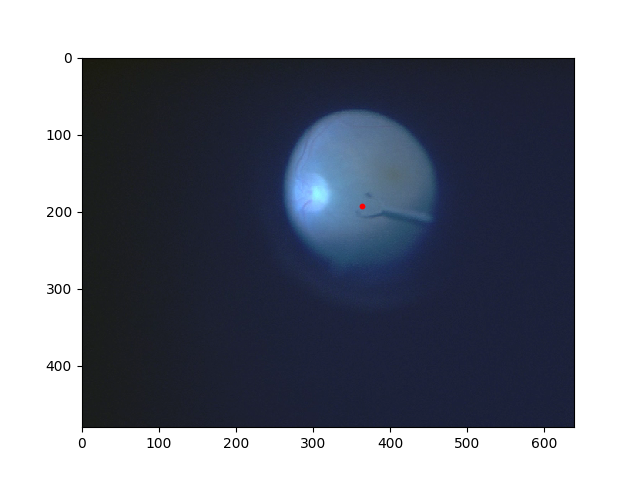
\includegraphics[width=0.25\textwidth]{figs/simplest/000271.png}
    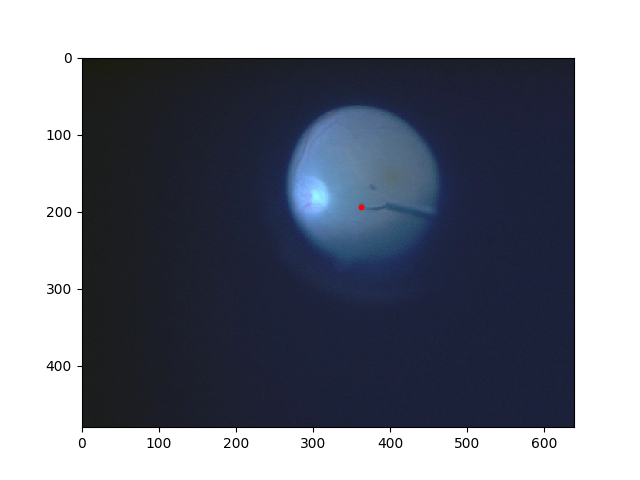
\includegraphics[width=0.25\textwidth]{figs/simplest/000272.png}
    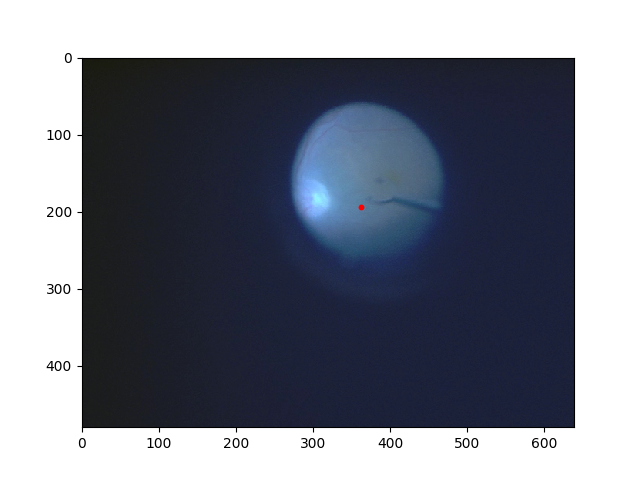
\includegraphics[width=0.25\textwidth]{figs/simplest/000273.png}
    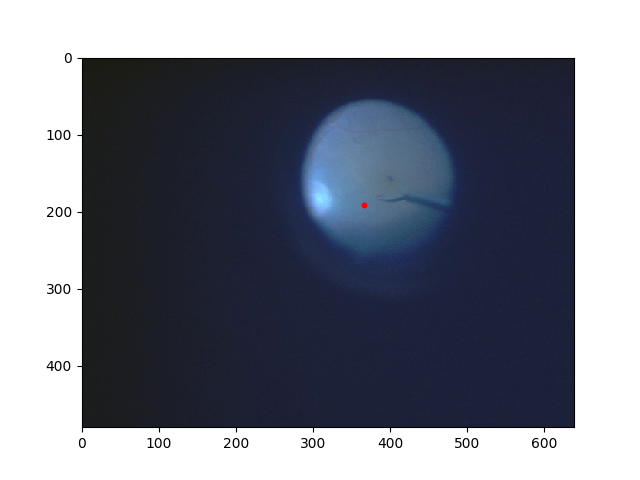
\includegraphics[width=0.25\textwidth]{figs/simplest/000274.png}
\end{figure}

\end{frame}


% ---------------------------------------------------------------------------------
%\begin{frame}{Genome assembly}%{Sequence read assembly and the need for scaffolding}
%\begin{figure}
%    \centering
%    \caption*{General workflow, \tiny{Vijay Lakhujani, Biostars, 2017}}
%    \includegraphics[height=0.5\textheight]{/home/exserta/Documents/master_project_noelle/journal_club/presentation/figs/GenomeAssembly.png}
%
%    \centering
%    \includegraphics[clip, trim={50 270 210 125},height=0.25\textheight]{/home/exserta/Documents/master_project_noelle/journal_club/presentation/figs/repeats_reads.pdf}
%\end{figure}
%\end{frame}


\end{document}